\chapter*{Introduction}
\addstarredchapter{Introduction} %Sinon cela n'apparait pas dans la table des matières
\markboth{Introduction}{Introduction} % headers


\section*{Contexte}
Ces dernières années, le domaine des drones s'est considérablement développé. En effet, de nombreux progrès ont été réalisés dans la conduite de vols autonomes, lesquels permettent de réaliser de nombreuses tâches longues, répétitives ou dangereuses, de manière plus sûre que des avions ou des systèmes télépilotés. Les drones ont fait leurs preuves dans de nombreuses applications civiles, alors qu'ils étaient auparavant conçus à des fins de surveillance et d'opération dans le secteur militaire. Tout leur intérêt réside dans leur capacité à se maintenir stabilisé sans intervention humaine. Ainsi, les opérateurs peuvent se concentrer sur la mission, sans devoir consacrer une grande attention au pilotage du drone. 

La possibilité d'utiliser des systèmes de vols autonomes dans le secteur civil a été rendue possible par l'accessibilité croissante, proposée par l'industrie, de solutions à faible coût pour les applications d'imagerie aérienne. Ainsi, ce sont dans des domaines aussi variés que l'agriculture de précision,  l'inspection des infrastructures civiles ou encore les opérations de sécurité que les drones autonomes sont aujourd'hui mobilisés, devenant alors un riche sujet de recherche.

La miniaturisation des équipements électroniques et mécaniques est à l'origine de l'essor d'une classe de drones de plus en plus petits. Souvent qualifiés de \textit{Micro Air Vehicle} (MAV) ou de \textit{Unmanned Aerial Vehicle} (UAV), leur petite taille leur permet d'intervenir dans des espaces confinés ou contraints. Ils n'ont, cependant, qu'une charge utile restreinte, souvent limitée à l'emport d'une caméra ou d'un colis de faible masse. Leur faible autonomie restreignant leur usage, la recherche s'est alors concentrée sur une solution permettant d'optimiser leur utilisation. En cela, les drones à décollage et atterrissage verticaux (\textit{Vertical take-off and landing}; VTOL) répondent aux exigences.
\nomenclature[]{\(VTOL\)}{Drones à décollage et atterrissage verticaux (\textit{Vertical Take-Off and landing})}
\nomenclature[]{\(MAV\)}{Micro drone (\textit{Micro Air Vehicle})}
\nomenclature[]{\(UAV\)}{Drone autonomes (\textit{Unmanned Aerial Vehicle})}

Dans l'ensemble des VTOL, plusieurs architectures existent et seront détaillées dans la section \ref{sec:archConvertible}. Toutefois, nos travaux se sont concentrés sur les classes des \textit{tailsitters} et des \textit{freewings}.

\subsection*{Phases d'un vol}
De nombreux travaux ont été menés sur les \textit{tailsitters}, avec l'objectif de couvrir l'intégralité du domaine de vol. Ce dernier est constitué des phases de vol suivantes :
\begin{enumerate}
    \item Décollage vertical
    \item Transition entre le vol stationnaire et le vol d'avancement
    \item Vol d'avancement
    \item Transition entre le vol d'avancement et le vol stationnaire
    \item Atterrissage vertical
\end{enumerate}


Bien que l'on puisse observer une symétrie entre la phase \raisebox{.5pt}{\textcircled{\raisebox{-.9pt} {1}}} et \raisebox{.5pt}{\textcircled{\raisebox{-.9pt} {5}}}, qui correspondent au décollage et à l'atterrissage vertical, une différence fondamentale est notable. Lors du décollage, la vitesse du drone engendrera un flux d'air sur l'aile, orienté dans le même sens que le flux d'air généré par les hélices. Cependant, lors de l'atterrissage, le flux d'air va se trouver inversé, le drone devant descendre, ce qui engendrera une vitesse opposée à la direction du flux d'air des hélices. Cette inversion génère une instabilité qui doit être compensée par le contrôleur.

Le vecteur $\overrightarrow{W}$ représente la perturbation de vent qui peut affecter le vol sur l'intégralité des cinq phases de vol. Toutefois, on observe que dans les phases de décollage \raisebox{.5pt}{\textcircled{\raisebox{-.9pt} {1}}}, de transition \raisebox{.5pt}{\textcircled{\raisebox{-.9pt} {2}}} et \raisebox{.5pt}{\textcircled{\raisebox{-.9pt} {4}}} et d'atterrissage \raisebox{.5pt}{\textcircled{\raisebox{-.9pt} {5}}}, le drone offre une grande surface verticale sujette au vent. Ainsi, il est nécessaire de traiter l'impact du vent sur cette architecture.

\begin{figure}[ht!]
    \centering
        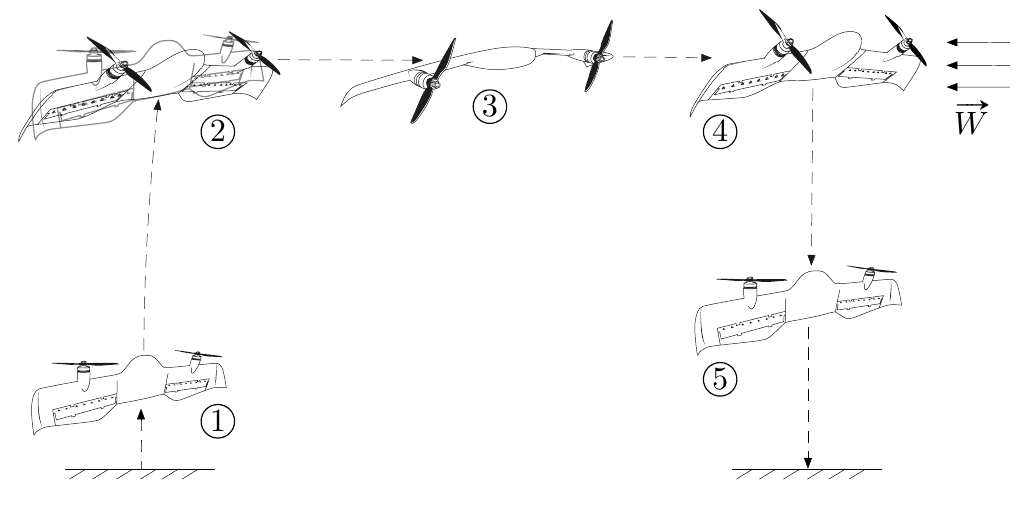
\includegraphics[width=0.8\columnwidth]{figures/darko_transition.png}
        \caption{Phases de vol d'un drone \textit{tailsitters}, DarkO.}
        \label{fig:darko_flight}
\end{figure}

\subsection*{Maquettes}

De nombreuses maquettes réelles ont été assemblées dans le but de réaliser des vols expérimentaux. Citons en exemples le \textit{tailsitter} à double rotor appelé «~T-Wing~» \cite{Stone2002PreliminaryDO, TWing2008}, le \textit{tailsitter} appelé «~MavIon~» \cite{oatao14575}, ou le «~JLion~» et le «~KH-Lion~» \cite{8003167}. Ces trois maquettes sont illustrées sur la figure \ref{fig:maquettetailsitter}.

\begin{figure}[ht!]
    \centering
    \resizebox{.9\textwidth}{!}{%
    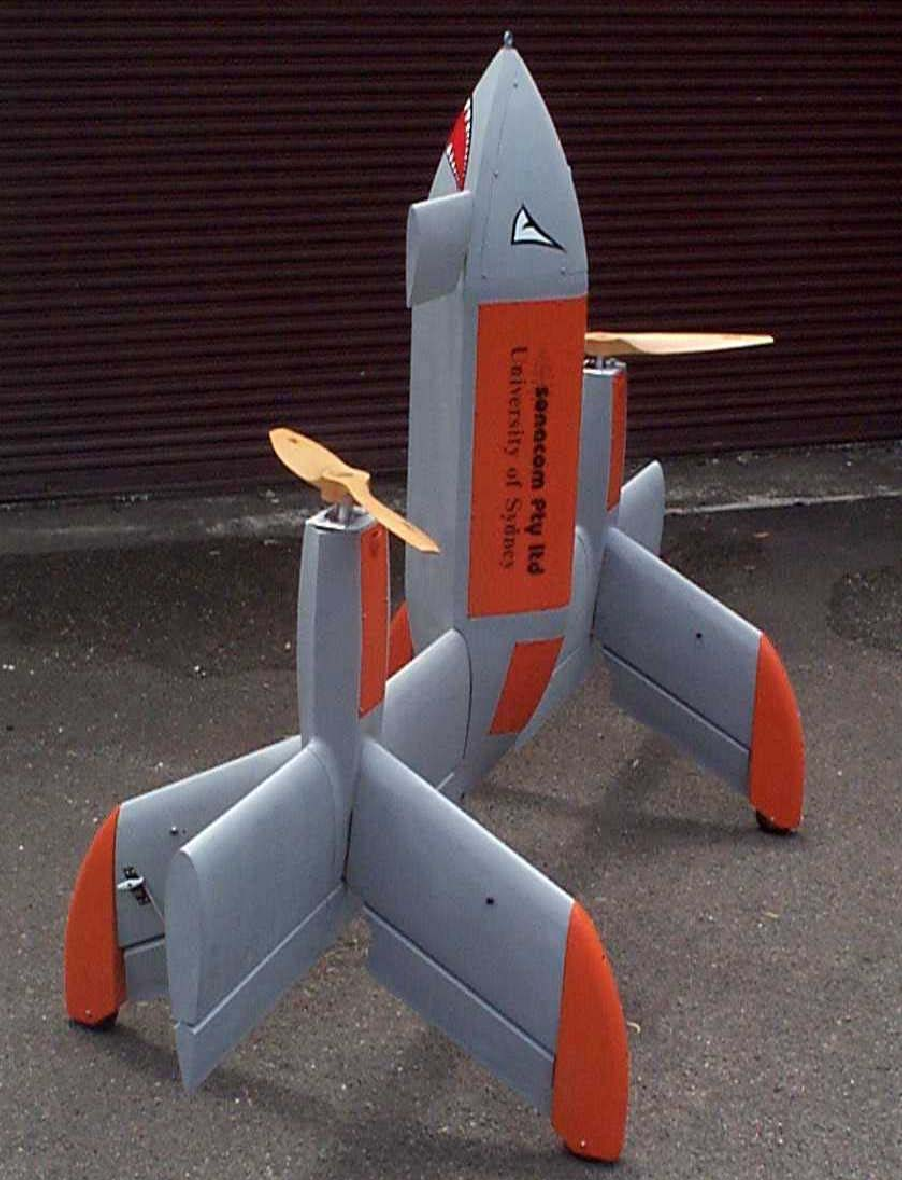
\includegraphics[height=3cm]{figures/T-Wing.png}
    \quad
    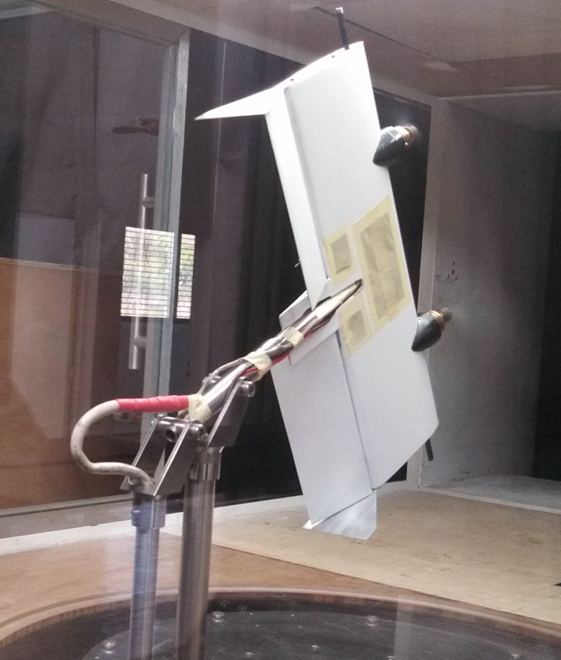
\includegraphics[height=3cm]{figures/mavionWindtunel.png}
    \quad
    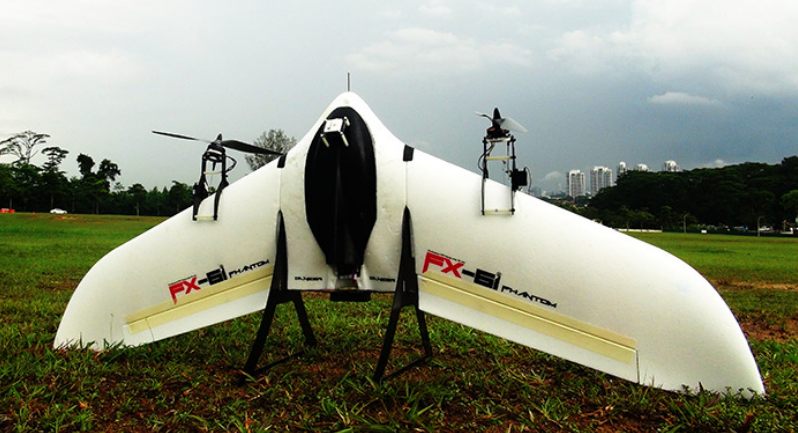
\includegraphics[height=3cm]{figures/KHlion.png}
    }
    \caption{Maquette «~T-Wing~», «~MavIon~» et «~KH-Lion~».}
    \label{fig:maquettetailsitter}
\end{figure}

Ces drones partagent une architecture similaire basée sur une aile supportant deux moteurs sur le bord d'attaque et soufflant deux élevons situés sur le bord de fuite. Cette architecture offre une plus grande robustesse que les \textit{tiltrotors}, composés de pièces mobiles (ce qui les rend plus fragiles) et d'un actionneur puissant pour faire tourner l'ensemble moteur-hélice.
La complexité inhérente à ces architectures nécessite un travail de modélisation en raison des nombreuses non-linéarités et couplages impliqués, en particulier en termes de modélisation des effets aérodynamiques. Dans ce contexte, l'interférence aérodynamique entre l'aile fixe et les rotors a été modélisée dans \cite{droandi_zanotti_gibertini_grassi_campanardi_2015, Simmons2022, aerospace5030079}, et les forces et moments d'hélice générés à des angles d'attaque élevés sont abordés dans \cite{Fernandez2023}. Cependant, ces modèles sont complexes algorithmiquement et ne sont que partiellement utilisables pour la conception des commandes. 

Un autre point important est la représentation de l'attitude du drone. Aussi, il est possible de représenter son orientation par des angles d'Euler \cite{4177650, 5415267, 8003165}, ce qui permet une compréhension intuitive. Toutefois, une singularité apparaît dans certaines phases de vol. Compte tenu de la grande manœuvrabilité, il est préférable de représenter l'attitude par un quaternion unitaire, ce qui élimine toute singularité \cite{8027691}. De nombreuses publications modélisent les effets aérodynamiques générés par les hélices en fonction de l'angle d'attaque et l'angle de dérapage \cite{Escareno07, ChiappinelliNahon2018}. 
Il est possible de choisir un autre modèle pour les interactions aérodynamiques entre les moteurs, les ailes et les élevons, comme présenté dans \cite{lustosaHal-03035938}. La technique de modélisation présentée dans \cite{lustosaHal-03035938} permet de disposer d'un modèle global couvrant l'ensemble de l'enveloppe de vol, grâce à ce que l'on appelle l'approche $\Phi$-théorie. Bien que cette dernière ne permette pas de prédire la chute brutale de la force de portance avec un angle d'attaque croissant (qui est causée par un flux d'air turbulent) \cite{tal2022global}, elle permet de représenter le drone avec suffisamment de précision pour capturer le comportement lors de manœuvres agressives. 



% Actuellement, nous pouvons mentionner deux types d'architectures de commande ayant fonctionné sur ce tailsitter. La première est basée sur une inversion incrémentale non-linéaire de la dynamique du drone (\textit{Incremental Non-linear Dynamic Inversion}, INDI) \nomenclature[]{\(INDI\)}{Inversion incrémentale non-linéaire  (\textit{Incremental Non-linear Dynamic Inversion})} et la seconde est basée sur une technique sans modèle (\textit{Model free control}, MFC). \nomenclature[]{\(MFC\)}{Commande sans modèle (\textit{Model free control})}

Les deux architectures sur lesquelles se sont concentrées nos recherches sont celles de DarkO, un \textit{tailsitters} et de Colibri, un \textit{freewings} basé sur une aile inspirée de DarkO, en rotation libre autour d'un fuselage qui sera maintenu horizontal.


\section*{Question de recherche}

Comme expliqué précédemment, lors des phases de décollage et d'atterrissage, le drone est vertical (voir figure~\ref{fig:darko_flight}), ce qui engendre une grande sensibilité aux perturbations. Il semble pertinent de concentrer nos travaux sur l'étude de la robustesse des drones convertibles face au vent.
Notre étude se focalise sur la recherche d'un contrôleur de vol unifié, pour une architecture de drone fortement non-linéaire et couplée, sur l'intégralité du domaine de vol, en environnement perturbé.

\section*{Objectifs fixés pour la thèse}
Les objectifs fixés sont pluriels : il s'agira d'étudier le comportement d'un drone \textit{tailsitters} en environnement perturbé en présence de saturation des actionneurs pouvant engendrer des cycles limites. Nous utiliserons la linéarisation pour extraire la dynamique du drone autour de l'ensemble des points d'équilibre. Nous étudierons la précision des linéarisations face aux nombreuses non-linéarités du modèle. 

De nos linéarisations, de notre compréhension du fonctionnement du drone et des limites analysées, il s'agira de proposer des architectures de commande basées modèle pour un drone \textit{tailsitters} permettant d'assurer une désensibilisation aux perturbations de vent. L'intérêt d'une architecture basée modèle est la possibilité de certification de ce type d'architecture. 

Pour finir, nous souhaitons utiliser des capteurs pour mesurer les perturbations en avance de phase pour les rejeter (sonde 5 trous, micro, Pitot, etc.). La connaissance d'une perturbation en amont de son impact sur le drone peut être un point clé dans la diminution de son impact. La mesure associée à un modèle peut être un moyen d'agir en anticipation plutôt qu'en réaction. Une action en anticipation pourrait se traduire par une modification de l'état du drone avant l'arrivée de la perturbation pour en minimiser son impact. À l'inverse qu'une action en réaction est une gestion de la perturbation suite à une modification de l'équilibre du drone (déplacement ou modification de son orientation) qui intervient après que la perturbation ait impacté le drone.  

Au vu des contraintes des \textit{tailsitters}, l'installation de capteurs de mesure de vent implique le développement d'une nouvelle architecture permettant l'installation d'un capteur capable de mesurer les perturbations sur l'intégralité du domaine de vol.


\section*{Plan et contribution}
Notre exposé commencera par une description générale des architectures de drone convertible (Chapitre~\ref{chap:generalites}), avec une présentation des avantages et des inconvénients ainsi que leur mode de fonctionnement. Une description générale de la modélisation, de l'actionnement et des lois de commande proposée sur les \textit{tailsitters} et les \textit{freewings} introduira nos propos sur ces architectures.

Le chapitre \ref{chap:model} détaillera le modèle non-linéaire d'un drone \textit{tailsitters}, DarkO, à partir des travaux de \cite{lustosaHal-03035938} et de \cite{olszaneckibarthHal-02542982}. Nous proposons un modèle simplifié pour les basses vitesses, ainsi que le détail des équilibres stationnaires en présence ou non de vent. De ces équilibres, nous présenterons la dynamique linéarisée du drone paramétrée par deux scalaires, le vent horizontal et vertical. Ce modèle étant le point de départ de chacun de nos travaux, il se retrouve expliqué dans \cite[Chapitre 2]{sansouStage} et \cite[Section II]{sansouECC} dans la condition de vent nulle, dans \cite[Section 2]{SANSOUACA} avec des conditions de vent non nulle et dans \cite[Section II]{sansouTCST} sous sa forme la plus complète.

Le chapitre \ref{chap:hybrid} fera l'objet d'une proposition de loi de commande hybride permettant d'augmenter le domaine de stabilité d'une loi linéaire avec une loi de commande non-linéaire basée sur une direction de zéro moment. Ces travaux ont été publiés dans  \cite{sansouStage} et \cite{sansouECC}.

Le chapitre \ref{chap:3DOF} permettra de décrire une maquette expérimentale utilisée pour évaluer les performances d'une loi de commande basée sur une architecture proportionnelle dérivative. Cette loi est un retour de sortie permettant de stabiliser une position stationnaire en présence de vent. Cette maquette restreint les degrés de liberté classiques d'un drone pour se concentrer sur la réjection de perturbation de vent, grâce à un changement d'incidence de la maquette. La description de la loi de commande, son optimisation et les résultats sont disponibles dans \cite{SANSOUACA}.

Le chapitre \ref{chap:LMI} propose une méthode d'obtention des gains de la boucle fermée différente basée sur les inégalités linéaires matricielles et la théorie de Lyapunov. L'ensemble de l'optimisation sera réalisé à l'aide de la dynamique linéarisé du drone autour de la condition de vent nulle. Ce contrôleur sera testé sur une maquette à six degrés de liberté en environnement contrôlé.

Le chapitre \ref{chap:6DOF} étendra le contrôleur proposé dans le chapitre \ref{chap:3DOF} pour stabiliser la dynamique complète d'un drone \textit{tailsitter}. La méthode d'obtention des gains du contrôleur est basée sur un algorithme itératif permettant de maintenir la complexité algorithmique, tout en identifiant les conditions de vol critiques. Les travaux ont été publiés dans \cite{sansouTCST}.

Le chapitre \ref{chap:colibri} propose une nouvelle architecture de \textit{freewing}. Cette dernière est inspirée d'un \textit{tailsitter} sur lequel on adjoint un fuselage pendulaire en rotation libre de manière à le maintenir horizontal dans toutes les configurations de vol. Nos travaux se sont concentrés sur l'obtention d'un modèle de simulation basé sur une dynamique multicorps. Des résultats de simulation et expérimentaux ont été proposés, basés sur un contrôle non-linéaire et publiés dans \cite{sansouICUAS}.




